\chapter{Marco teórico} % Main chapter title
\label{capitulo2} % Change X to a consecutive number; for referencing this chapter elsewhere, use \ref{capitulo2}
\section{Competencias académicas y su evaluación}
La creciente profesionalización trajo al campo educativo elementos evaluativos tales como calidad, equidad, competitividad, eficiencia, y eficacia; junto con ellos surgieron las competencias, que pasaron a jugar papel importante en el contexto educativo. En la formación de profesionales, resalta la necesidad de reflexionar sobre los aprendizajes que se ofrecen en las instituciones educativas, las cuales deben servir al estudiante para ser útil a la sociedad, que es su entorno inmediato \citep{kuh_using_2015}. En otras palabras, la competencia es la capacidad de un buen desempeño en contextos complejos y auténticos. Se basa en la integración y activación de conocimientos, habilidades, destrezas, actitudes y valores.

De esa necesidad va surgiendo la idea de las evaluaciones orientadas a competencias. Cabe resaltar cómo se desenvuelve el aprendizaje basado en competencias usando aplicaciones como herramientas para la evaluación de estudiantes, mediante el análisis de los aportes que introduce la tecnología en este campo, que modifican significativamente las prácticas tradicionales \citep{carriveau_connecting_2016}.

Uno de los factores de motivación relevantes para el aprendizaje es la evaluación. Cada actividad ofrece a los estudiantes la oportunidad de conocer cuáles son sus resultados de aprendizaje en lo que se refiere al \enquote{qué} se ha aprendido y al \enquote{cómo} habría podido hacerse. Cualquier proceso de evaluación debería ser diseñado teniendo en cuenta este principio básico.

En un sistema de gestión de evaluaciones basado en competencias, los encargados hacen evaluaciones según las evidencias obtenidas de diversas actividades de aprendizaje, que definen si un estudiante alcanza o no los requisitos recogidos por un conjunto de indicadores en un determinado grado. Una evaluación por competencias asume que pueden establecerse indicadores posibles de alcanzar por los estudiantes, que diferentes actividades de evaluación pueden reflejar los mismos indicadores \citep{barrio_minton_evaluating_2016}.

La evaluación por competencias ofrece nuevas oportunidades a los estudiantes al generar entornos significativos de aprendizaje que acercan sus experiencias académicas al mundo profesional, y donde pueden desarrollar una serie de capacidades integradas y orientadas a la acción, con el objetivo de ser capaces de resolver problemas prácticos o enfrentarse a situaciones cotidianas \citep{carriveau_connecting_2016}.

Hoy día existen herramientas que ayudan al alumno a potenciar su aprendizaje y algunas de ellas son los sistemas de gestión de aprendizajes y los sistemas de gestión de evaluaciones basadas en competencias, cuyas diferencias se mostrarán a posteriori.
\section{Sistemas de gestión de aprendizajes}
Las plataformas LMS\footnote{de sus siglas en inglés, Learning Management System, que significa en español sistema de gestión de aprendizajes.} son espacios virtuales de aprendizaje orientados a facilitar la experiencia de aprendizaje a distancia y permite una cómoda interacción de profesores y alumnos. En la misma se pueden hacer evaluaciones, intercambiar archivos y participar en foros y chats, además de otras herramientas de interacción estudiante a profesor.

La centralización y automatización de la gestión del aprendizaje es una de las principales características de los LMS. La plataforma puede ser adaptada tanto a los planes de estudio de la institución como a los contenidos y estilo pedagógico de la misma.

El usuario se convierte en el protagonista de su propio aprendizaje a través del autoservicio y los servicios guiados por los tutores o profesores mediante la herramienta. Además, permite utilizar los cursos desarrollados por terceros, personalizando el contenido y reutilizando el conocimiento adquirido. Además, posee prestaciones y características que hacen que cada plataforma sea adecuada según los requerimientos y necesidades de los usuarios.

Los LMS que almacenan información de programas académicos no involucran el aspecto de resultados pedagógicos en sus estructuras de datos o procesos de aprobación. Sin embargo, no es capaz de soportar competencias de institución de manera completa, aunque puede hacerlo por medio de plugins pero es un soporte superficial y no cubre con todas las necesidades de las universidades comunitarias del estado de California. Por lo que se utilizan los AMS para evaluar a los alumnos.\citep{aalst_workflow_2004}.
\section{Sistemas de gestión de evaluación basadas en competencias}
Un AMS es un sistema, generalmente basado en tecnologías web, que permite a la institución la recolección, el manejo, y reporte de datos relacionados a las evaluaciones, por lo general basadas en competencias, del estudiante. Los AMS basadas en competencias permiten a la institución y a los educadores listar sus competencias, guardar, y mantener datos para cada competencia, facilitar conexiones a competencias similares de la institución, y generar reportes\citep{cartwright2009student}.

Los AMS permiten que las competencias sean enlazadas a nivel institucional, departamental, de programas, y de división. Esta estructura permite examinar la competencia
acorde al nivel que pertenece. Una representación común de este tipo de enlace es el mapa curricular\citep{oakleaf_choosing_2013}. Algunos de estos sistemas de manejo de evaluaciones generan sus propios mapas curriculares.

Varios sistemas de manejo de evaluaciones comerciales existen; incluyendo Blackboard Learn, Campus Lab, eLumen, LiveText, TaskStream, TracDat/Webfolio, Waypoint Outcomes y WEAVEOnline. Además de estas aplicaciones comerciales para manejo de evaluaciones también existen otras hechas por las propias instituciones para manejar sus datos de evaluaciones.

Mientras que cada AMS tiene un conjunto diferente de capacidades, todas manejan, mantienen, y permiten generar reportes de los datos de las evaluaciones. Generalmente, teniendo como ejemplo los distintos sistemas, los AMS tienen una estructura jerárquica basada en unidades organizacionales (programas, departamentos, escuelas, colegios o la misma institución), por lo tanto, las metas y/o las competencias también se ven adaptadas a esta estructura.

\subsection{Capacidad de evaluación}
La característica más importante de todo AMS es la capacidad de soportar evaluaciones con sus diferentes tipos de evaluación. Por ejemplo, algunos AMS se centran soportar evaluaciones acumulativas; mientras que otros permiten además el seguimiento de las evaluaciones formativas. Además, las capacidades de evaluación apoyadas por una AMS pueden residir en una escala de la unidad.

Algunos AMS permiten evaluaciones a nivel de estudiante. Un número cada vez mayor de las AMS apoyan la documentación, desarrollo o aplicación de criterios de evaluación específicos, más comúnmente a las rúbricas que se aplican a los productos creados por los estudiantes.

Como una faceta adicional, muchos AMS permiten evaluaciones para vincularse con las normas educativas y profesionales, de modo que la información de evaluación de múltiples unidades puede ser adherido como datos de reportes.

\subsection{Alineación de capacidades}
Una importante característica de cualquier AMS es la habilidad de enlazar competencias con cualquier nivel de la institución u organización.

Primeramente, algunos AMS permiten que las competencias sean enlazadas a nivel institucional, departamental, de programas, de división. Esta estructura permite examinar la competencia acorde al nivel que pertenece. Una representación común de este tipo de enlace es el mapa curricular. Algunos de estos sistemas de manejo de evaluaciones generan sus propios mapas curriculares.

Un sistema de manejo de evaluaciones o AMS es un sistema web que provee soporte a iniciativas de mejora continua educacionales de instituciones y competencias de aprendizaje que necesitan las evaluaciones. [bibliografía pendiente] Un AMS puede ser levantado y utilizado para mantener y alcanzar altos estándares de calidad y cumpliendo los requisitos de acreditación. [bibliografía pendiente]
Esta evaluación es un proceso complejo que requiere la contribución y la retroalimentación de todo el personal, profesores y alumnado de un centro de educación superior. El sistema AMS facilita la esquematización, la recopilación de pruebas, documentación y presentación de las contribuciones que cada uno de los programas académicos de la institución y los servicios de apoyo hace la consecución de los objetivos de calidad y eficacia institucionales.

Un ciclo de evaluación completo incluye la coordinación, la planificación, la medición, la reflexión y la toma de acción del proceso de evaluación de la institución enteras, programas o cursos.
\section{Diferencias entre LMS y AMS}
Por lo general, en las universidades norteamericanas utilizan los AMS y LMS para mejorar el proceso de evaluación de sus estudiantes. Sin embargo, para las personas que no están familiarizadas con estos sistemas pueden quedar ambiguas las diferencias entre estos sistemas de aprendizaje. Estas diferencias se encuentran sumarizadas y tabuladas en la tabla \ref{comparacion_ams_lms}.

\begin{table}[H]
\centering
\caption{Comparación de características entre plataformas AMS y LMS.}
  \label{comparacion_ams_lms}
  \resizebox{\columnwidth}{!}{%
	\begin{tabular}{lllcc}
		\toprule
		\multicolumn{3}{l}{Características}                                                                     & AMS       & LMS       \\
		\midrule
		\multicolumn{3}{l}{Soporte de evaluaciones a los estudiantes.}                                          & $\checkmark$         & $\checkmark$         \\
		\multicolumn{3}{l}{Soporte de evaluación colectiva.}                                                    & $\checkmark$         &           \\
		\multicolumn{3}{l}{Diferentes tipos de rúbricas para evaluaciones.}                                     & $\checkmark$         &           \\
		\multicolumn{3}{l}{Permite acceder a cursos realizados por terceros (aula virtual para el estudiante).} &           & $\checkmark$         \\
		\multicolumn{3}{l}{Permite la evaluación de desempeño estudiantil.}                                     & $\checkmark$         &           \\
		\multicolumn{3}{l}{Permite generar reportes de cursos, progresos, etc.}                                 & $\checkmark$         & $\checkmark$         \\
		\multicolumn{3}{l}{Soporte de presupuestos (solicitud de profesores, coordinadores, etc.).}             & $\checkmark$         &           \\
		\multicolumn{3}{l}{Soporta competencias de aprendizaje del estudiante o Student Learning Outcomes.}     & $\checkmark$         &           \\
		\multicolumn{3}{l}{Soporte de alineación de competencias.}                                              & $\checkmark$         &           \\
		\multicolumn{3}{l}{E-portfolio y evaluación de proyectos.}                                              & $\checkmark$         & $\checkmark$         \\
		\multicolumn{3}{l}{Soporte de comunicación entre estudiantes y profesores (foro).}                      &           & $\checkmark$         \\
		\multicolumn{3}{l}{Soporte de evaluación sumativa y formativa.}                                         & $\checkmark$         &           \\
		\multicolumn{3}{l}{Software distribuido y desarrollado libremente.}                                     &           & $\checkmark$         \\
		\bottomrule
	\end{tabular}
	}
\end{table}

Los LMS permiten al estudiante a una capacitación flexible a distancia sin limitaciones de horarios con costos reducidos. Además, como es una plataforma intuitiva, permite a las personas con nivel de conocimiento básico en informática un aprendizaje constante y actualizado a través de la interacción entre alumnos y profesores. En cambio, los AMS son más bien utilizados para evaluaciones de las competencias de los alumnos que como vínculo entre el alumno y el profesor mediante un aula virtual, y permiten la mejora continua del aprendizaje estudiantil.

Los LMS permiten la integración de competencias mediante herramientas externas, pero de una manera superficial en comparación a los AMS.
\section{Programas de estudio}
En términos generales, se puede definir un programa de estudios como una herramienta educativa que regula y ordena el proceso de enseñanza-aprendizaje a desarrollar en una unidad de aprendizaje determinada, orientando las actividades que profesor y alumno han de llevar a cabo para el logro de los objetivos planteados en dicha unidad, en relación con los objetivos del plan de estudios, de tal manera que el egresado concluya su carrera con el perfil deseado. En pocas palabras, es un esquema organizado de los contenidos situados dentro de una determinada unidad de aprendizaje\citep{lalor_ensuring_2017}.

El termino \enquote{unidad de aprendizaje} sustituye al de \enquote{asignatura} o \enquote{materia} que evocan los tradicionales cursos unidisciplinarios, generalmente teóricos y sobrecargados de información. Un programa resume las características de la unidad de aprendizaje, su contenido mínimo obligatorio, y sus objetivos, principalmente.

En la primera etapa de diseño curricular, se requiere la elaboración de la propuesta de los programas para su aprobación de parte de las autoridades con la colaboración de las academias y, de ser necesario, con la asesoría de externos de la unidad académica.

\subsection{Proceso de diseño curricular} \label{procesoCurricular}
Para aquellas personas ajenas al entorno educativo, en específico aquellas que no forman parte del proceso de diseño curricular puede ser un tanto complejo el proceso de creación y revisión de material curricular en las instituciones. En la actualidad, un formulario de creación o revisión de competencias, cursos, y programas debe pasar por una serie de evaluadores (figura \ref{flujo_autoridades}) que son los encargados de revisar y verificar que los datos sean válidos.
\begin{figure}
\centering
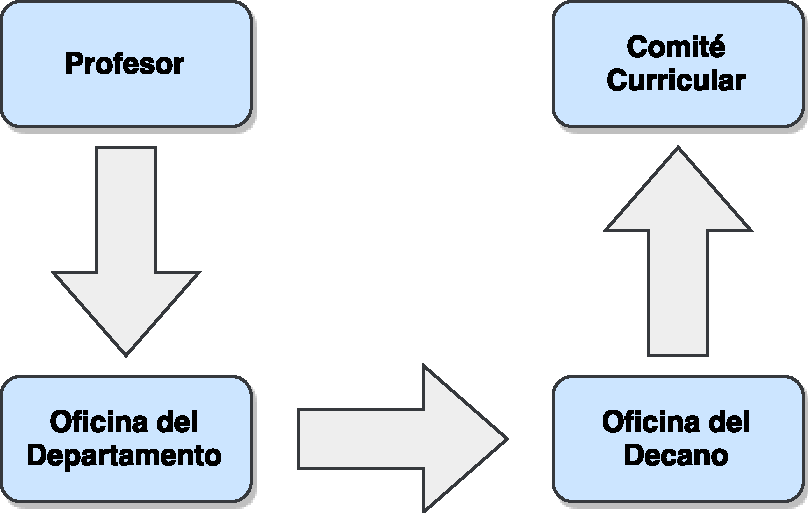
\includegraphics[scale=0.5]{Capitulos/MarcoTeorico/Imagenes/flujo_autoridades}
\caption{Flujo de creación y revisión de propuestas.}
  \label{flujo_autoridades}
\end{figure}

Hoy día el estado de California cuenta con un patrón de definición de cursos y programas donde la misma sirve como guía para el desarrollo de propuestas para material académico de las universidades. Dicho estándar además contiene una taxonomía de programas e indica cuál es el flujo para la revisión de las propuestas, donde todo es establecido en el PCAH\footnote{de sus siglas en inglés, Program and Course Approval Handbook, que significa en español manual de aprobación de cursos y programas.}.

El flujo inicia con el profesor o encargado del curso o programa, una vez completado pasa por la mesa de recepción donde se verifica que cumpla con el estándar estatal para luego pasar por la oficina departamental y la oficina del decano para su revisión de contenido. Una vez revisado y con el visto bueno de ambas oficinas pasa por una última revisión por parte de la oficina curricular para ser registrada en los sistemas de gestión curricular (figura \ref{course_creation_flow}).

Es un proceso que se hace con formularios en papel donde el profesor o encargado del curso o programa tiene que completar los campos requeridos para que el estado de California cuente al curso como válido. Dicho proceso tiene varias deficiencias como las que estaremos citando a continuación:
\begin{itemize}
	\item La creación o revisión puede tomar meses debido a los formularios que son completados a mano y requieren de revisión de varias oficinas.
	\item Es un flujo de una sola dirección, eso quiere decir que si es que una de las oficinas rechaza el formulario debe volver a iniciar el flujo.
	\item Se puede producir cuellos de botella en los diferentes puntos de revisión.
\end{itemize}

Una vez ya registrado en los sistemas de gestión curricular es accesible de manera pública para el uso de las universidades del estado de California. De esta manera, si una institución académica posee un sistema de gestión de evaluaciones y quiere incluir los cursos o programas válidos para el estado tiene ingresar los nuevos datos del sistema de gestión curricular uno a uno como se puede apreciar en la figura \ref{after_creation}.

\begin{figure}
\centering
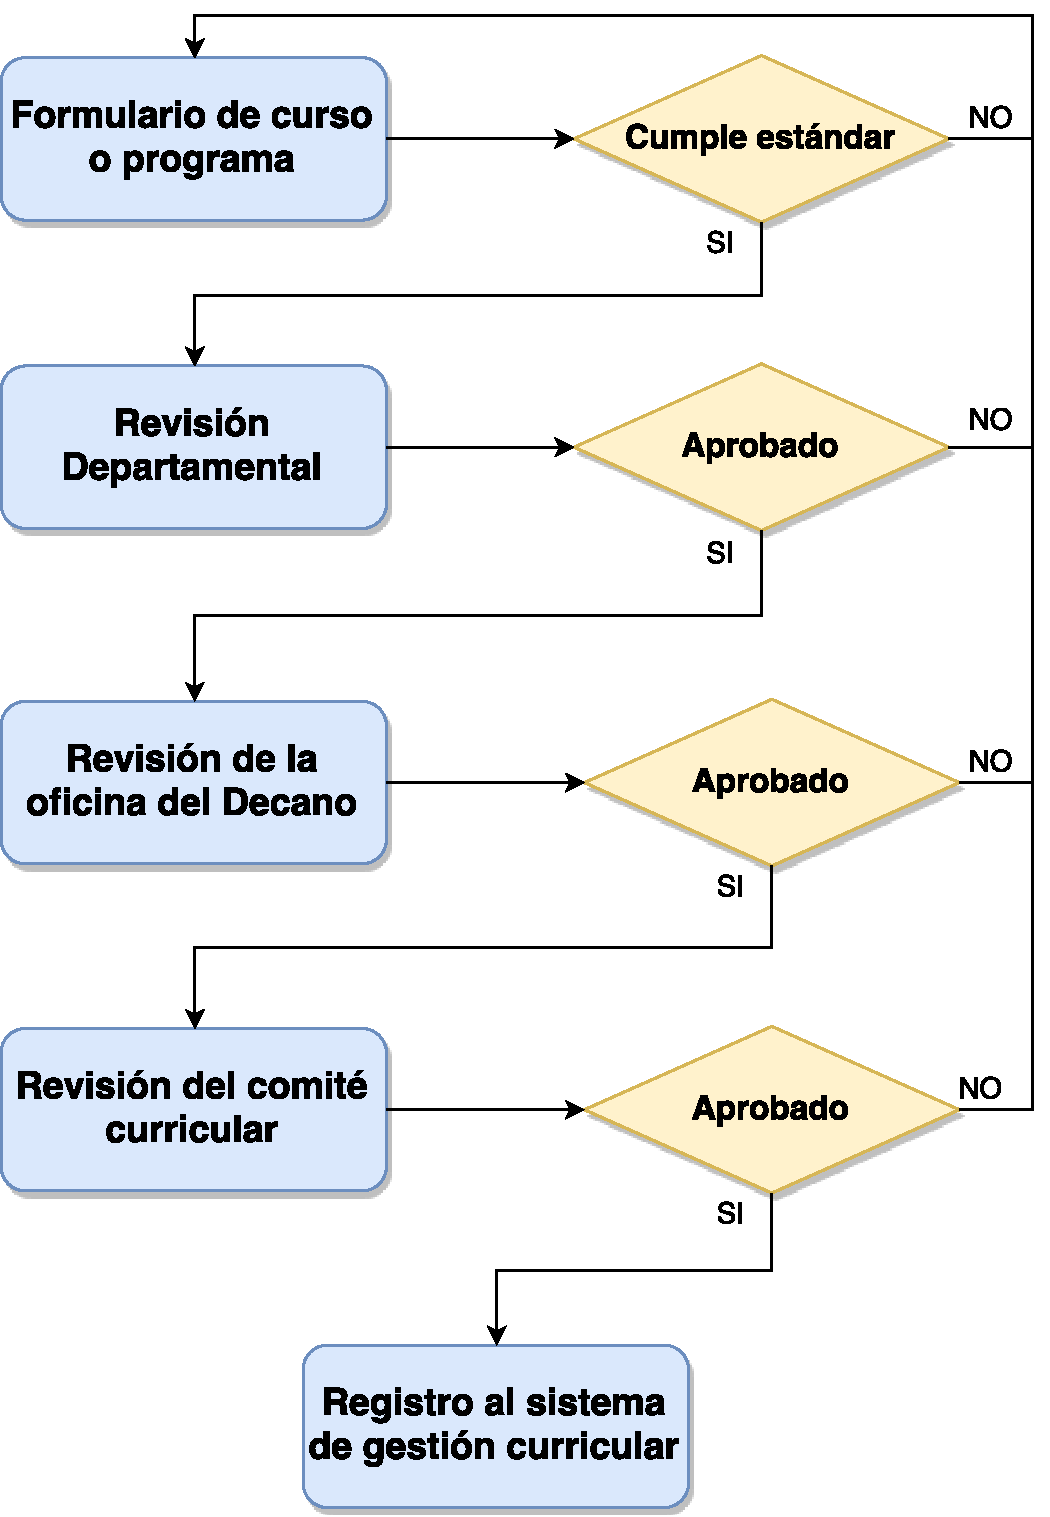
\includegraphics[scale=0.5]{Capitulos/MarcoTeorico/Imagenes/course_creation_flow}
\caption{Flujo actual de diseño de cursos, programas y competencias.}
  \label{course_creation_flow}
\end{figure}

\begin{figure}
\centering
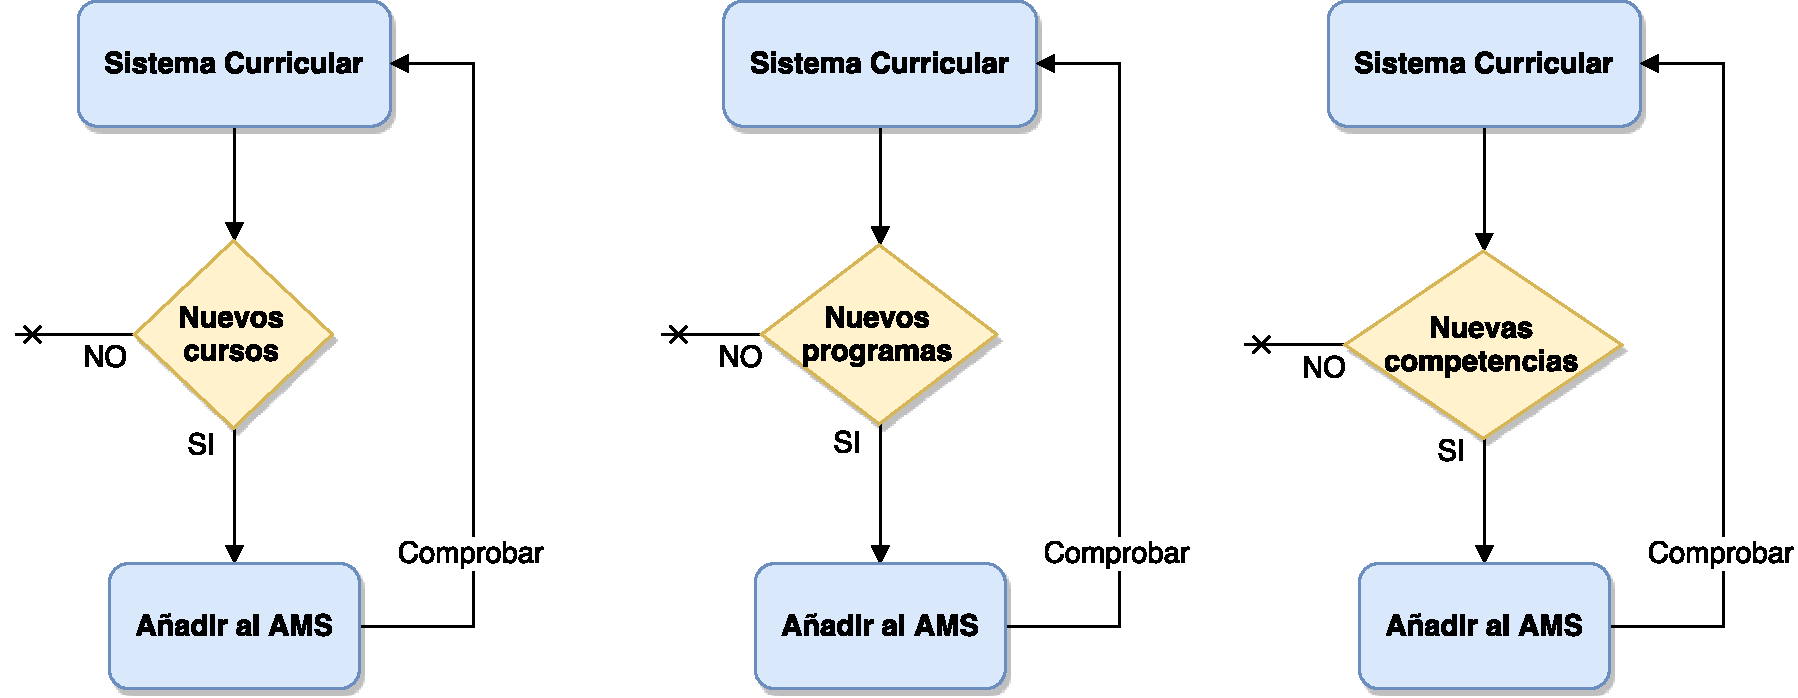
\includegraphics[width=125mm,scale=1]{Capitulos/MarcoTeorico/Imagenes/after_creation}
\caption{Esquema de tipos de computación en la nube.}
  \label{after_creation}
\end{figure}
\section{Sistemas de gestión curricular}
Un CMS \footnote{de sus siglas en inglés, Curriculum Management System, que significa sistema de gestión curricular} es un aplicación automatizada que apoya todo el proceso curricular, desde la planificación hasta la implementación y evaluación. Posee una interfaz única y cohesiva en línea que permite proponer, crear, evaluar, revisar, aprobar y aplicar cursos, programas y competencias\citep{harden2001amee}.

Curriculum es una mezcla sofisticada de estrategias educativas, contenido del curso, resultados de aprendizaje, experiencias educativas y evaluación. Esta visión amplia de un CMS se deriva del ambiente actual de educación elemental y secundaria que es impulsado por los estándares de contenido de cursos obligatorios federales y estatales, y la necesidad de auditorías continuas de currículo\citep{west2000technology}.

En los enfoques actuales del desarrollo de Curriculum por lo general gira en torno a los comités curriculares. Un comité curricular departamental comienza el proceso de desarrollo curricular considerando como entrada cualquiera de los aspectos mostrados en la figura \ref{diseno_curricular}.

\begin{figure}[H]
\centering
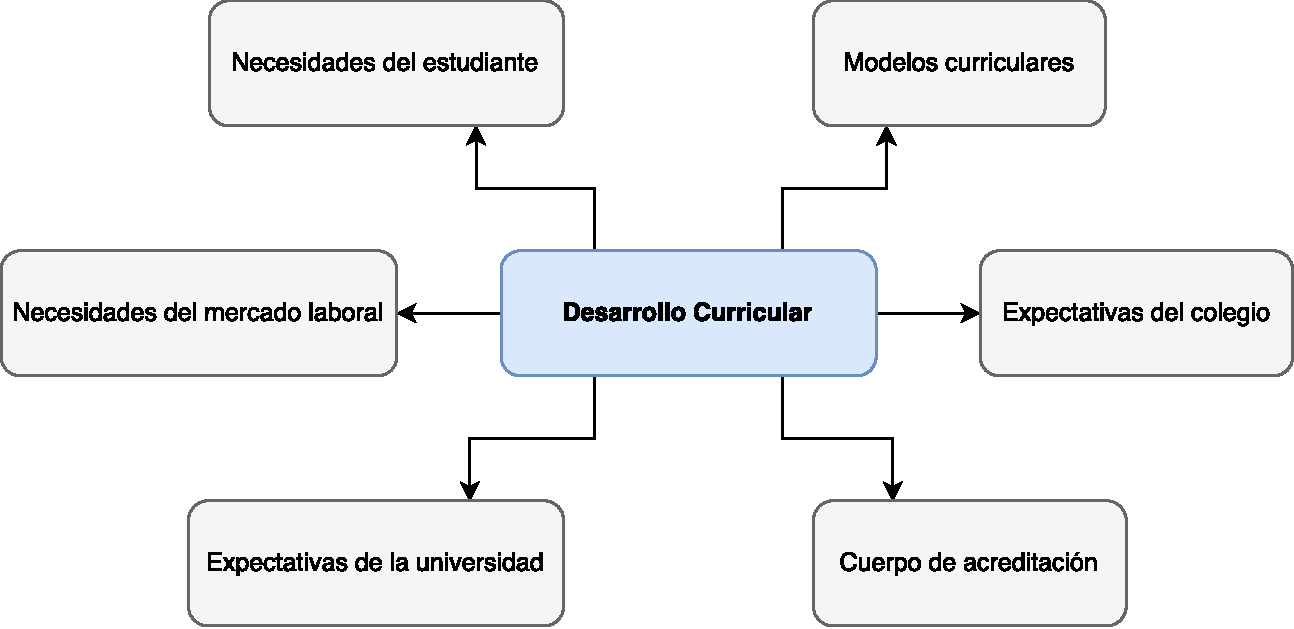
\includegraphics[width=125mm,scale=1]{Figuras/diseno_curricular}
\caption{Esquema de diseño curricular y sus variables determinantes.}
  \label{diseno_curricular}
\end{figure}


Dichos aspectos, sin embargo, sólo se consideran en un alto nivel de abstracción basado en la comprensión tácita de los miembros del comité sobre la disciplina.
\section{Aplicaciones web}
La necesidad de ejecución de operaciones complejas de manera remota y portable, tales como el uso de software sin depender de la potencia del hardware del usuario, la disponibilidad de uso en múltiples plataformas, y muchas otras, han guiado al desarrollo y evolución de las aplicaciones web. En las ciencias de la computación, una aplicación web es un software con arquitectura cliente-servidor donde el cliente (o interfaz de usuario) corre en un navegador web\citep{net_app_architecture}.

Los usuarios acceden a la aplicación utilizando un navegador web y no es necesario descargarse ningún tipo de software adicional, ya que la aplicación se ejecuta en el servidor. Para esclarecer el panorama, la lógica de la aplicación web se ejecuta remotamente, y el navegador web sólo se limita a la representación de los datos.

La evolución de las aplicaciones web ha crecido tan vertiginosamente que además de ofrecer una multitud de servicios, mejoran la UX a través de interfaces gráficas impactantes e intuitivas para los usuarios\citep{myers_past_2009}.
\section{Cloud computing}
Casi toda solución de infraestructura remota es llamada hoy día con el termino de computación en la nube o simplemente la nube.

La computación en la nube es una metáfora para abastecimiento y consumición de recursos de infraestructura. El nivel de abstracción ofrecida por la nube puede variar de hardware virtual a complejos sistemas distribuidos, debido a que los recursos están disponibles a demanda en enormes cantidades y pagados por uso\citep{wittig_amazon_2016}.

La infraestructura remota o nube puede ser manejada por una organización abierta para uso público, o puede ser privada, donde una nube que virtualiza y comparte la infraestructura con una sola organización o híbrida como son mostrados en la figura \ref{cloud_types}.

\begin{figure}[H]
\centering
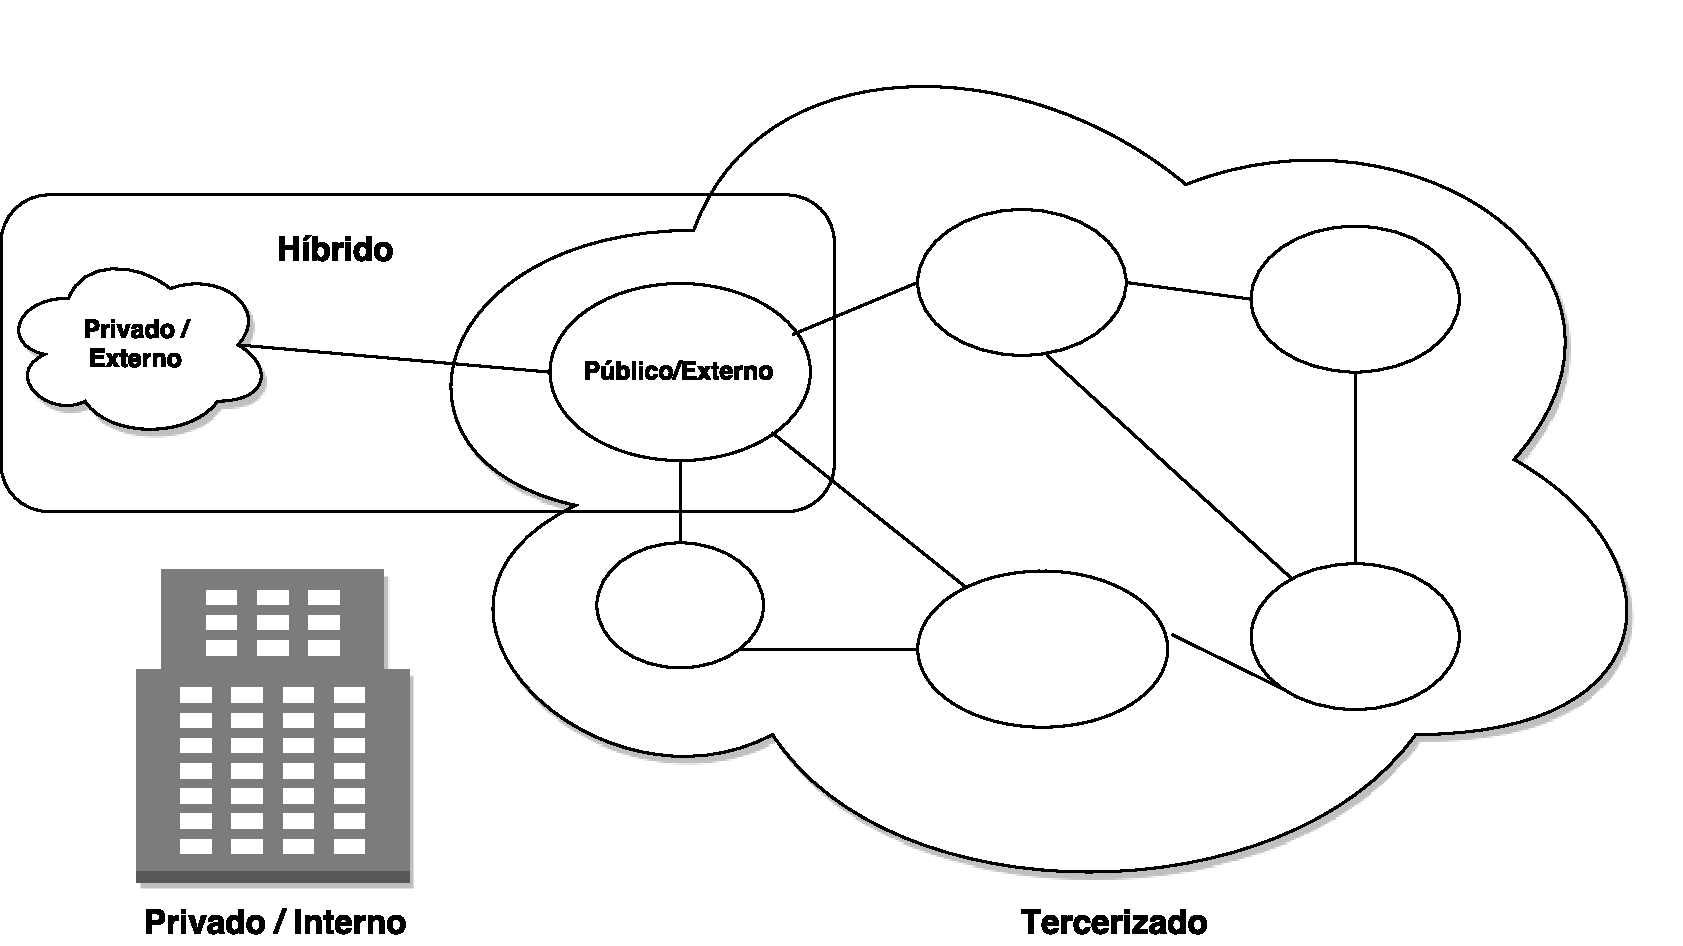
\includegraphics[width=125mm,scale=1]{Figuras/cloud_computing_types}
\caption{Esquema de tipos de computación en la nube.}
  \label{cloud_types}
\end{figure}
\section{Software as a Service}
SaaS\footnote{de sus siglas en inglés, Software as a Service, que significa en español software como servicio.}, es un paradigma de entrega de software donde la misma se encuentra alojada por lo general en la nube y se entrega como servicio a través de Internet a un gran número de usuarios a través de un modelo de suscripción. Se trata de un modelo de entrega de negocio en el que tanto la aplicación y el alojamiento son gestionados y compartidos con varias empresas, que alquilan y utilizan los servicios de aplicaciones de forma centralizada\citep{gupta_software_2014}.

El software como servicio es equivalente a servicios de proveedores externos que manejan todo mantenimiento, personalización, actualización y cobro para los servicios que su cliente utiliza de manera mensual o anual. El proveedor se encarga de ofrecer el software basado en un conjunto de códigos y datos definidos junto a las diferentes configuraciones para los diferentes clientes. Los suscriptores al servicio acceden a la aplicación con la sensación de que son los únicos usuarios de la aplicación. Sin embargo, los cambios de configuraciones como cambios de datos, flujo de trabajo, interfaz y el flujo de negocio son realizados de manera masiva y transparente para ellos\citep{kumar_cloud_2012}\citep{kang_web_2012}.

También existen otras opciones como PaaS\footnote{de sus siglas en inglés, Platform as a Service, que significa en español plataforma como servicio.} e IaaS\footnote{de sus siglas en inglés, Infraestructure as a Service, que significa en español infraestructura como servicio.}.

\subsection{Características}
Entre las características relevantes de las aplicaciones SaaS, y las que las remarcan como aplicaciones bien construidas, son desarrolladas a la medida, escalables y soportan multitenancy\footnote{En español se conoce como multiples clientes inquilinos, se refiere cuando varios clientes pueden utilizar la misma instancia.}. No todas las aplicaciones SaaS comparten todas las características, pero las más comunes son las siguientes: 

A nivel de la configurabilidad, las aplicaciones con esta característica poseen el mismo código base y provee a instancias con múltiples opciones de configuración tal que cada cliente pueda tener sus propias configuraciones de software únicas y pueda tener la sensación de que es el único usuario en utilizar la aplicación. Esta es la clave del éxito para las aplicaciones SaaS\citep{jadeja2012cloud}. Por ejemplo, cada cliente puede tener configurado su sitio para que muestren fondos de pantallas o logos en las páginas de inicio de sesión o páginas principales que ellos especifican. Esta característica también puede ser llamada personalización de la aplicación.

Desde la óptica del concepto de Multitenancy, una sola instancia de la aplicación corriendo puede servir a una cantidad de clientes. Los diferentes modelos de datos que están disponibles para soportar SaaS son las bases de datos aisladas, arquitectura de bases de datos aisladas compartidas y la construcción de datos\citep{lee2012web}. Utilizando la arquitectura multitenant los proveedores de aplicaciones SaaS pueden innovar de forma sencilla y ahorrar tiempo valioso gastado en mantener varias versiones de código deprecado y/o desactualizado\citep{kang2011design}.

Por otro lado se tiene el criterio de escabilidad, el cual es una de las características más complicadas de agregar a una aplicación SaaS debido a su elevado costo. La escalabilidad es soportada por la virtualización, pero teniendo en cuenta el costo y el problema de complejidad muchas veces el desarrollador de la aplicación no se complica con esta característica\citep{li2012cooperative}.

Además, aparte de las características mencionadas anteriormente, algunos beneficios que poseen las aplicaciones con arquitectura SaaS son las siguientes: \citep{li2012cooperative}\citep{ma2007business}\citep{chou2008software} 
\begin{itemize}
	\item Las aplicaciones SaaS pueden ser utilizadas por los usuarios por medio de sus navegadores Web. Esto ahorra en costos operacionales para el usuario junto con los requerimientos de hardware mínimo, por lo tanto, reduce el costo que el usuario necesita gastar en hardware.  Además de los costos de mantenimiento, costos de licencias del software también son minimizados.
	\item Mejor utilización de recursos, debido a que los recursos requeridos por las aplicaciones con arquitectura SaaS son mínimos.
	\item El avance de la tecnología Web permite que los proveedores de SaaS se ubiquen en el extranjero y también ofrezcan servicios de alta calidad. De esta manera, permite a los usuarios de la aplicación ahorrar en infraestructura.
	\item Usualmente, las soluciones SaaS residen en entornos en la nube donde son escalables y poseen integración con otras ventajas SaaS. En comparación al modelo tradicional, los usuarios no tienen que comprar otro servidor o software.
\end{itemize}
\section{Metodología Ágil de desarrollo de software}
La metodología Ágil envuelve un enfoque para la toma de decisiones en los proyectos de software, que se refiere a métodos de ingeniería del software basados en el desarrollo iterativo e incremental, donde los requisitos y soluciones evolucionan con el tiempo según la necesidad del proyecto. Los métodos tradicionales, como Waterfall, pretenden ser capaces de modelar completamente el dominio del problema de entrada y luego esperar que se produzcan pequeños cambios (o inclusive ninguno)\citep{davis_agile_2015}. Los métodos ágiles asumen que el cambio es inevitable, por lo que abordan el desarrollo de software de tal manera a facilitar la adaptación de los nuevos requisitos mientras vayan surgiendo.

Las metodologías ágiles, en comparación a otras metodologías de desarrollo, ofrecen un modelo de diseño flexible que fomenta al desarrollo evolutivo. Los desarrolladores trabajan en pequeños módulos cada vez y la retroalimentación proveída por el cliente ocurre simultáneamente en el desarrollo. Además, la metodología puede ser bastante útil en situaciones donde los objetivos finales del proyecto no están claramente definidos donde los requisitos del cliente se clarificarán gradualmente a medida que el proyecto avance.

El uso de la metodología ágil como método de entregas de las características del módulo entra como requisito no funcional.

\subsection{Historias de usuario}
Las historias de usuario conforman la parte central de muchas metodologías de desarrollo ágil, tales como XP\footnote{de sus siglas en inglés, eXtreme Programming, que significa en español programación extrema}, Scrum, entre otras. Estas definen lo que se debe construir en el proyecto de software, tienen una prioridad asociada definida por el cliente de manera a indicar cuales son las más importantes para el resultado final. Son divididas en tareas y su tiempo es estimado por los desarrolladores.

Por lo general, se espera que una estimación de tiempo de cada historia de usuario se sitúe entre horas y el tiempo máximo de iteración. Estimaciones superiores a este tiempo máximo son indicativas de que la historia es muy compleja y debe ser dividida en varias historias.

Una historia de usuario es una representación de un requisito escrito en una o dos frases utilizando el lenguaje común del usuario\citep{davis_agile_2015}. Ellas son utilizadas para la especificación de requisitos acompañadas de las discusiones con aquellos y las pruebas de validación.

Cada historia de usuario debe ser limitada. La metodología estipula que las mismas deben ser escritas por los clientes. Son una forma rápida de administrar los requisitos sin tener que elaborar gran cantidad de documentos formales y sin requerir de mucho tiempo para administrarlos.

Las historias de usuario deben ser:
\begin{itemize}
    \item \textbf{Independientes:} de ser necesario, combinar las historias dependientes o buscar otra forma de dividir las historias de manera que resulten independientes.
    \item \textbf{Negociables:} la historia en sí misma no es lo suficientemente explicita para considerarse un contrato, la discusión con los usuarios debe permitir esclarecerse y éste debe dejarse explicito bajo la forma de pruebas de validación.
    \item \textbf{Valoradas:} Los intereses de los clientes y de los usuarios no siempre coinciden, pero en todo caso, cada historia debe ser más importante para los clientes que para el desarrollador.
    \item \textbf{Pequeñas:} las historias grandes son difíciles de estimar e imponen restricciones sobre la planificación de un desarrollo iterativo. Generalmente se recomienda la consolidación de historias muy cortas en una sola historia.
    \item \textbf{Estimables:} las historias completas en requerimientos de parte del equipo de desarrollo y de parte del cliente son estimables. Y por lo tanto, el equipo debe estar cómodo de puntuar las historias de usuario.
    \item \textbf{Verificables:} las historias de usuario cubren requerimientos funcionales, por lo generalmente son verificables. Cuando sea posible, la verificación debe automatizarse, de manera que pueda ser verificada en cada entrega del proyecto.
\end{itemize}

Las iniciales de estas características, con sus nombres en inglés, forman la palabra INVEST, que significa “inversión”. Es porque toda historia de usuario, si se construye bien, es una inversión.

Al momento de implementar las historias, los desarrolladores deben tener la posibilidad de discutirlas con los clientes. El estilo sucinto de las historias podría dificultar su interpretación, podría requerir conocimientos de base sobre el modelo, o podría haber cambiado desde que fue escrita.

Cada historia de usuario debe tener en algún momento pruebas de validación asociadas, lo que permitirá al desarrollador, y más tarde al cliente, verificar si la historia ha sido completada. Como no se dispone de una formulación de requisitos precisa, la ausencia de pruebas de validación concertadas abre la posibilidad de discusiones largas y no constructivas al momento de la entrega del producto.

\subsection{Épicas}
Una épica es esencialmente una historia de usuario de un tamaño mucho mayor, siempre superior al tiempo de iteración máximo, y tiene como propósito el de asociar historias de usuario individuales relacionadas con un propósito de más alto nivel que cumplir. La misma es, por lo general, muy grande para que un equipo del proyecto pueda trabajar directamente sin partir en diversas historias de usuario\citep{cobb2015project}.

El uso de las épicas en proyectos de gran tamaño ayuda a organizar tareas complejas en un tipo de estructura para que la interrelación de historias de usuario esté bien entendida. Por lo tanto, el diseño de épicas en el proceso de desarrollo es fundamental antes de comenzar cualquier proyecto.
\section{Interacción humano-computador}
En HCI definen la funcionalidad y la usabilidad de los sistemas que se desarrollan, donde la funcionalidad de un sistema es definida por un conjunto de acciones o servicios que son proveídas a los usuarios, sin embargo, el valor de la funcionalidad es verificada cuando es eficientemente utilizada por el usuario \citep{shneiderman_designing_2010}. La usabilidad de un sistema con cierta funcionalidad es el rango y grado por el cual el mismo puede ser utilizada de manera eficiente y adecuada para cumplir ciertas metas para ciertos usuarios. La eficiencia de un sistema es alcanzada cuando se cumple un balance entre la usabilidad y la funcionalidad \citep{nielsen_usability_2010}.

HCI es un diseño que debe producir un ajuste entre el usuario, la máquina y los servicios requeridos con el fin de lograr un balance óptimo entre la calidad y la eficiencia de los servicios.

La definición de la estrategia de UI\footnote{de sus siglas en inglés, User Interface, que significa en español experiencia de usuario.} es importante para una mejor usabilidad del sistema, donde este proceso debería comenzar antes que el diseño y desarrollo de las aplicaciones. Es la visión de una solución que necesite ser verificado con potenciales usuarios que prueben que necesite el mercado \citep{levy_ux_2015}.